\section{Repeating the controller comparisons}
The exploratory matrix identifies informative changes, but a single split cannot show their variability across query samples. We therefore repeat three settings on all ten primary splits: one outstanding read, ClosedCAP cap four, and the alternate address mapper. These change the opportunity for overlap, row lifetime and address-to-bank placement respectively. Each setting replays all five layouts at both footprints, for 300 additional runs.

\begin{table}[htbp]\centering\small
\caption[Repeated controller comparisons]{Query-aware cycle difference against BFS under three repeated controller settings. Each estimate uses ten matched splits with the same graph. Negative means fewer cycles.}\label{tab:repeated}
\begin{tabular}{lrrr}
\toprule
Setting & Bytes & $\Delta$ QA/BFS (\%) & 95\% interval \\
\midrule
Outstanding: 1 & 512 & -0.13 & [-0.14, -0.13] \\
Outstanding: 1 & 128 & -1.26 & [-1.30, -1.21] \\
ClosedCAP, cap 4 & 512 & +0.89 & [+0.79, +0.99] \\
ClosedCAP, cap 4 & 128 & +5.27 & [+5.15, +5.39] \\
Alternate mapper & 512 & -4.02 & [-4.28, -3.75] \\
Alternate mapper & 128 & -4.12 & [-4.26, -3.99] \\
\bottomrule
\end{tabular}

\end{table}
\begin{figure}[htbp]\centering
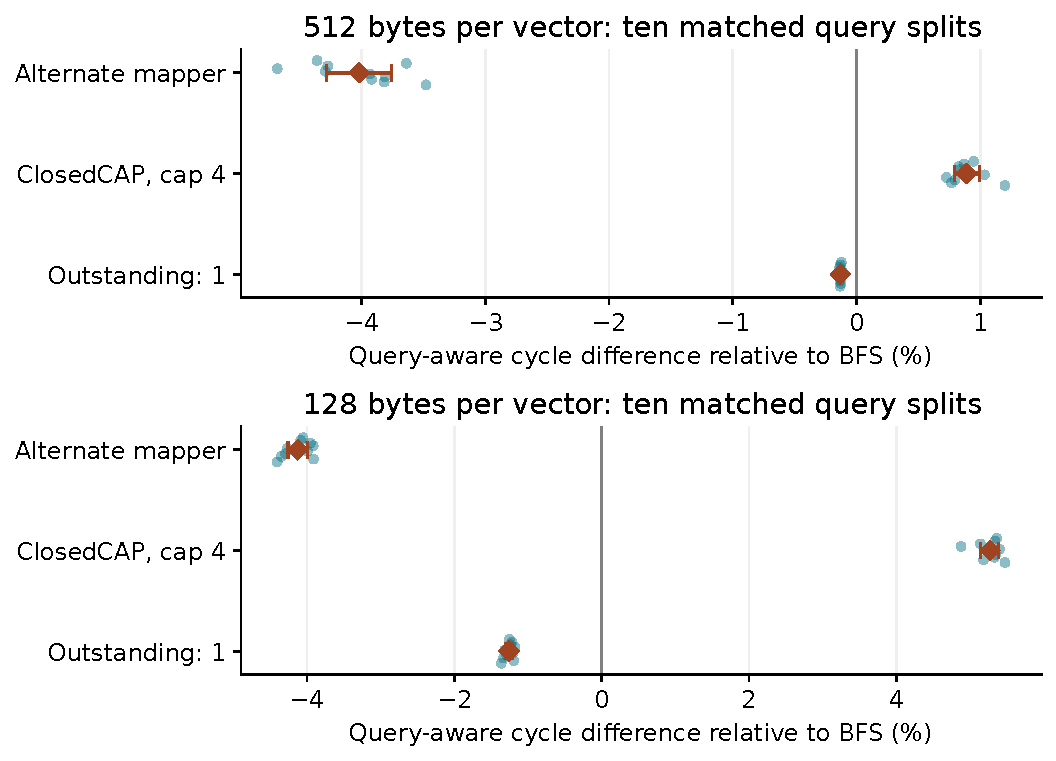
\includegraphics[width=\textwidth]{generated/robust_controllers.pdf}
\caption[Individual effects and paired intervals]{Individual split effects (small teal points) and mean with paired 95\% interval (orange diamond and bar). Showing the observations alongside the intervals makes their consistency and dispersion visible.}\label{fig:repeated}
\end{figure}

The query-aware/BFS sign is consistent across all ten splits in each repeated setting: query-aware is faster at both widths with one outstanding read and with the alternate mapper, and slower at both widths under cap four. The size of the effect also changes substantially, as Table~\ref{tab:repeated} shows. Under the alternate mapper, random placement is faster still than query-aware at 512 bytes in every split. A gain relative to BFS therefore does not identify the best layout among all controls.

The other controller settings and all training ablations retain their single-split interpretation. The repeated settings were chosen after inspecting the exploratory matrix; their ten splits include that original first split. This is a targeted robustness extension, not an independent confirmatory experiment. It strengthens the comparison under those specific interventions without sampling an architectural population.

\section{Changing the graph while preserving corpus IDs}
The previous repetitions share one constructed graph. The next experiment keeps the same 100,000 vectors but changes the structure used to search them. Graph seeds 101 and 102 vary HNSW's random construction with corpus insertion order fixed. A third alternative keeps graph seed 100 and shuffles insertion with seed 17. Each alternative uses query splits one through three and all five layouts at both footprints, adding 90 replays.

\begin{table}[htbp]\centering\small
\caption[Graph-construction robustness]{Query-aware/BFS cycle differences for four constructions on the same three query splits. The mean and minimum/maximum describe these observations; the range is not a confidence interval over possible graphs.}\label{tab:graphrobust}
\begin{tabular}{lrrr}
\toprule
Graph construction & Bytes & Mean $\Delta$ (\%) & Observed range (\%) \\
\midrule
Seed 100, corpus order & 512 & -0.341 & [-0.357, -0.331] \\
Seed 100, corpus order & 128 & +0.119 & [+0.034, +0.186] \\
Seed 101, corpus order & 512 & -0.247 & [-0.386, -0.062] \\
Seed 101, corpus order & 128 & -0.191 & [-0.267, -0.081] \\
Seed 102, corpus order & 512 & -0.268 & [-0.330, -0.212] \\
Seed 102, corpus order & 128 & -0.705 & [-0.798, -0.627] \\
Seed 100, shuffled order & 512 & -0.320 & [-0.499, -0.161] \\
Seed 100, shuffled order & 128 & +0.040 & [-0.057, +0.203] \\
\bottomrule
\end{tabular}

\end{table}

At 512 bytes, query-aware placement uses fewer cycles than BFS in every tested construction/split pair. At 128 bytes, the ranking changes: the reference graph's three-split mean is \GraphRefCompact\%, while seeds 101 and 102 give \GraphOneCompact\% and \GraphTwoCompact\%. Shuffled insertion has mean \GraphShuffleCompact\% and individual splits on both sides of zero. Thus the original 128-byte loss is not a stable property of the footprint alone. Query-split precision on one graph did not establish robustness to constructing another graph.

The reference row uses only those same three splits, making it comparable with the alternatives. Graph hashes confirm four distinct topologies, and repeated builds of each construction agree. Corpus IDs remain stable: changing insertion order does not redefine which vector a logical ID names, which vectors count as exact neighbours, or what identity placement means.

Recall across these graph/split conditions ranges from \GraphRecallMin\% to \GraphRecallMax\%. A changed graph can change the number of candidate evaluations and therefore total traffic. For this reason, Table~\ref{tab:graphrobust} compares layouts within each graph and split. Directly comparing absolute cycles from two different graphs would combine search-work and placement effects. These selected constructions expand the evidence beyond one topology, while leaving corpus and dataset generalisation open.

\section{Explaining the 128-byte layout reversal}
The main SIFT table contains a smaller version of the controlled paradox: query-aware placement gives more row hits than BFS at 128 bytes, yet slightly more cycles. To inspect that result, the command observers replay split one for both layouts with outstanding limits one and 64. Each case is run with the original mixed trace, vector requests only, and adjacency requests only. Query boundaries are preserved. Removing a request type is a diagnostic intervention, not an alternative complete HNSW execution.

\begin{table}[htbp]\centering\small
\caption[Command accounting for the layout reversal]{Query-aware minus BFS for the 128-byte diagnostic streams on split one. Negative counts mean fewer cycles or commands. The last two columns sum exactly to the cycle difference. Limit is the outstanding-read bound.}\label{tab:realcommands}
\begin{tabular}{rlrrrr}
\toprule
Limit & Stream & $\Delta$ cycles & $\Delta$ ACT & $\Delta$ commands & $\Delta$ no cmd. \\
\midrule
64 & Mixed & +2848 & -12516 & -25125 & +27973 \\
64 & Vectors & +3858 & -12401 & -24873 & +28731 \\
64 & Adjacency & +0 & +0 & +0 & +0 \\
1 & Mixed & -278960 & -12771 & -17009 & -261951 \\
1 & Vectors & -265883 & -12582 & -16435 & -249448 \\
1 & Adjacency & +0 & +0 & +0 & +0 \\
\bottomrule
\end{tabular}

\end{table}

For the mixed stream at limit 64, query-aware placement needs \MixedSavedACT{} fewer activations and \MixedSavedCommands{} fewer command-issue cycles. It nevertheless adds \MixedExtraNoCommand{} no-command cycles, leaving a net cost of \MixedDeltaCycles{} cycles. The vector-only case retains the reversal. The adjacency-only traces have the same addresses and order for both layouts and give identical results. Consequently, the effect is already present in vector service; it does not require a changed adjacency layout.

The vector placement also changes offered bank diversity: the mixed input spans \BfsOfferedBanks{} banks per complete 64-request window for BFS and \QAOfferedBanks{} for query-aware placement, on average. This is consistent with increased concentration accompanying row reuse. The observed command/no-command accounting establishes where the cycle difference lies; the input statistic and controlled concurrency experiment support the mechanism, without proving that bank diversity is its only cause.

Vector-only and adjacency-only times must not be added to predict mixed timing. Interleaving the streams changes which requests compete, which rows remain open and which timing delays overlap. The additive identity in Table~\ref{tab:realcommands} applies to command and no-command cycles of a single replay, not to separate component replays.

\subsection{Why a high hit percentage needs a denominator}
A 512-byte vector becomes sixteen consecutive 32-byte reads. In an illustrative uninterrupted access with a closed row initially, one read may require opening the row and the remaining fifteen may hit it: $15/16=93.75\%$. At 128 bytes, the analogous fraction is $3/4=75\%$. These are opportunities within one vector; they are not measured predictions because controller ordering, row state and intervening traffic can change classification.

\begin{table}[htbp]\centering\small
\caption[Within-vector and adjacency traffic]{Traffic composition averaged over the ten primary splits. The last two percentages use all emitted transactions as denominator. A within-vector follow-up is any transaction after the first transaction of that logical vector read. It is not automatically a row hit.}\label{tab:traffic}
\begin{tabular}{rrrr}
\toprule
Vector bytes & Reads/vector & Vector traffic (\%) & Within-vector follow-ups (\%) \\
\midrule
512 & 16 & 98.64 & 92.48 \\
128 & 4 & 94.78 & 71.09 \\
\bottomrule
\end{tabular}

\end{table}

The layout heuristic attempts to improve relationships between different vectors. Table~\ref{tab:traffic} shows why its effect can be small beside the locality already available inside each vector. Reporting the aggregate row-hit rate alone obscures that distinction. The consecutive-vector same-block diagnostic examines another denominator---transitions between distinct vector reads---and therefore cannot be substituted for the simulator's request-based percentage.
